\documentclass[a4paper, 11pt]{report}
\usepackage[T1]{fontenc}
\usepackage[utf8]{inputenc}
\usepackage{charter}
\usepackage[libertine]{newtxmath}
\usepackage{graphicx}
\usepackage[pdfa]{hyperref}
\usepackage{color}
\usepackage{setspace}
\usepackage{parskip}
\usepackage[a4paper, inner=0.5cm, outer=0.5cm, lmargin=3.0cm, rmargin=3.0cm,
tmargin=2.0cm, bmargin=2.1cm]{geometry}
\usepackage{listings}
\definecolor{dkgreen}{rgb}{0.1,0.5,0.1}
\definecolor{greengray}{rgb}{0.32,0.57,0.32}
\definecolor{orange}{rgb}{0.96,0.42,0}
\definecolor{lightblue}{rgb}{0,0.28,0.95}
\definecolor{background}{rgb}{0.995,0.995,0.995}
\lstset {
	frame=tb,
	language=java,
	aboveskip=3mm,
	belowskip=3mm,
	showstringspaces=false,
	columns=flexible,
	basicstyle={\small\ttfamily},
	numbers=none,
	backgroundcolor=\color{background},
	numberstyle=\tiny\color{drkgeen},
	keywordstyle=\color{lightblue},
	commentstyle=\color{greengray},
	stringstyle=\color{orange},
	breaklines=true,
	breakatwhitespace=true,
	tabsize=3
}
\setlength{\parindent}{0pt}

\begin{document}
\setstretch{1.20}
\title{Computer Networks 2 and Introduction to Cybersecurity}
\author{Marco Sgobino}
\maketitle
\tableofcontents

\part{Transmission Control Protocol internals}

\chapter{Basics}

\section{Brief recap of TCP}
TCP is a procotol that has the following properties,

\begin{itemize}
	\item allows \emph{connection between processes};
	\item is \emph{connection-oriented}: before transmitting data, a
		connection must be established \--- this is different to what
		IP protocol does in network layer, since in IP protocol there
		is no concept of connection, and messages are exchanged in
		packets;
	\item is \emph{reliable}: it assures all segments are correctly
		delivered through use of \texttt{ACK} mechanism, and \textbf{at
		most once} \--- again, this is different to IP layer, since IP
		packets are unreliable and there is no guarantee that they will
		be delivered, let alone in their correct ordering;
	\item offers a \emph{sliding window} mechanism for congestion control
		and stream control. This assures read and send buffers are
		well-optimized in both sender and receiver \--- this feature is
		much important since it allows fine-tuning the connection and
		avoiding waste of resources;
	\item is \emph{byte-oriented}: the byte stream is fragmented into
		multiple segments, and composed again after getting to
		destination \--- in this manner, huge payloads can be reliably
		delivered in multiple segments, each one having the correct
		order to the application.
\end{itemize}

The logical structure is the following one: there are two entities, client and
server. The client first authenticates to the server; after that, the server
opens a connection and client executes the send-receive loop. Both server and
client create a \emph{socket} $s$ (a UNIX-like file abstraction), and the
client connect $s$ to IP-srv, port-srv. The communication takes place on $s$ by
means of application protocol (applications will exchange data each other). The
connection is said to be \emph{reliable}: losses and packet loss are carefully
managed, and segments\footnote{\emph{Segments} refer to the particular kind of
package that TCP protocol exchange. Usually, in literature one could find the
term package referring to TCP segments; while this is not fully correct, it may
be acceptable when there is no ambiguity.} arrive in the same order as they are
sent.

A very simplified pseudo-code at client's side for TCP is as follows,

\begin{verbatim} int s; s := socket(...); 
connect(s, IP-srv, port-srv,...); 
...
send (s, msgl, ...); 
... 
msg2 := receive(s,...); 
... 
\end{verbatim}

where the notation \texttt{...} denotes possibly code in between two
instructions.

The logical structure at server side is quite different. A server creates
a socket $s1$, chooses a port number to bind to that socket, then it declares
willingness to accept connections on $s2$, and finally it awaits for connection
requests on $s2$. Basically, it creates two different sockets, the first to
accept a new connection, and the second one to actually manage the connection.
A server usually remains on \emph{sleep} until a connection is requested.

\begin{verbatim} 
s1 := socket(...);
bind(s1, portsrvm ...);
listen(s1,...);
s2 := accept(s1,...); // another socket 
... 
msg1 := receive(s2,...);
...
send(s2,msg2,...);
... 
\end{verbatim}

In TCP, communication is \emph{bidirectional}, with a pattern that depends on
the application protocol. The send-receive patterns heavily depend on the
application itself \--- browser send-receive sequences are very different from,
let's say, an e-mail client send-receive sequence. There is no guarantee that
two different application protocols will exchange a similar amount and kind of
TCP messages.

\subsection{TCP Implementation}

There are many differences between TCP and IP, set aside their abstraction
layer. IP operates between \emph{nodes}: it is \emph{connectionless},
\textbf{unreliable}, and is \emph{message-oriented}. The Maximum Transmission
Unit size of an IP packet is $MTU = 64KB$. TCP lies on top of IP, adopting
coutermeasures to overcome the unreliable aspects of IP.

TCP layers communicate between themselves in terms of \emph{segments}. A
segment is a \emph{message between TCP layers}, and contains a \emph{TCP
header} and \--- eventually \--- data \emph{payload}. Payload can either be $0$
bytes long or carry some information (wanted by the application layer). An
important property is that \emph{a TCP segment must be small enough to fit in a
single IP packet}, hence IP header and TCP segment size should be no greater
than $64KB$, the MTU of an IP packet.

A segment is thus composed by a IP header, whose payload is a TCP segment. The
TCP segment is in turn composed by a TCP header, followed by eventual
application data. Usually, IP header size is usually $20$ bytes, as well as TCP
header that is $20$ bytes. The IP datagram can be greater up to $64KB$, with
the first $40$ to $50$ bytes reserved to headers.

Segments can carry portions of data (for instance, in a video stream many
segments should be sent to client in order to carry enough information and let
application layer reconstruct the video correctly). For this reason, in
application layer, one application message could correspond to \emph{many
segments} in TCP layer, in \textbf{both} directions. In fact, at TCP level
multiple segments are usually required in order to send a single
application-level message. Each TCP layer represents a connection as (<id>,
<state>). The <id> is the <IP-local, port-local, IP-remote, port-remote>, while
the <state> refers to the state of the TCP connection. Conceptually there is a
single table storing both <id> along with connection <state>.

IP addresses are extracted from the IP header, while port numbers are extracted
from TCP header. Packets are thus sorted accordingly. The connection <state>
includes information on the \emph{Maximum Segment Size} (MSS), which is the
maximum size of the \emph{data part} of a segment that the other part is
willing to achieve. The MSS is negotiated upon connection opening \--- this
value is, in practice, identical in both direction and is not arbitrary. In
most cases and for historical reasons, there are only $2$ possible values that
depend whether the connection:

\begin{itemize}
    \item lies on different networks (through internet), MSS is $536$ bytes
        (MTU=576), that is the maximum segment size that can fit in the
        smallest possible packet;
    \item lies on the same network (for example, ethernet), MSS is $1460$ bytes
        (MTU=1500), which corresponds to ethernet MTU minus the IP header and
        TCP header.
\end{itemize}

The core idea is that each segment must be \emph{sufficiently small} to fit in
one packet along the full path, in order to prevent fragmentation.

\subsubsection{Establishing a TCP Connection}

At the beginning of a TCP connection, $3$ segments are needed, while $2$
segments are needed to close it.

FIXME DNS -> To forge it, must change IP address to
response AS WELL AS copying Transaction ID of request

\section{TCP Architecture}

TCP has many different implementations, depending mostly on OS of choice.
Several variants of its components have been written, with many of them largely
optional. TCP works in segments. Execution flow at application level works
independently and unpredictably with respect to the TCP-level flow. When an
application sends something, multiple TCP packages must be exchanged. The
sequence of bytes will be copied to a buffer (sliding window) and the
\texttt{send()} function is, for example, invoked \--- the time in which a
segment is sent is \emph{unpredictable}, \emph{unrepeatable} and depends on
many things. This means that application cannot \emph{deterministically
predict} the exact time in which the transmission will occur \--- instead, the
TCP layer will deliver the payload at a specific time determined by the
protocol\footnote{However, many more effects can concur: for instance, the
Operating System may not be ready to send a segment, or may be busy with other
resources.}.

On TCP, many events can provoke a transmission:

\begin{itemize}
    \item application invokes \texttt{send()} \--- in this case, the data in
        send's call argument will be inserted into the proper transmission
        buffer, and it will be transmitted somewhere in the (immediate) future;
    \item application invokes \texttt{receive()} \--- this way, we will see in
        detail that the TCP protocol provides a \emph{response} that
        \emph{acknowledges} the receipt of a segment;
	\item TCP layer \emph{receives a segment} \--- the same as above;
	\item a \emph{timeout} occurs;
\end{itemize}

Each of the above will trigger a transmission either immediately or
\emph{withing a maximum predefined time} (in the case of a timeout, for
instance). When a TCP layer is touched from above or below, \textbf{it reacts
by transmitting a segment}. Transmission may occur \emph{even if there is no
useful data to transmit} (e.g. the transmission buffer is empty) \-- in that
case, a segment will only carry the header, which has information useful to the
protocol itself. Upon transmission, TCP may deliver a varying number of bytes,
ranging from empty up to a number of bytes \emph{larger than Maximum Segment
Size} ($536$ in Internet network, $1460$ for same Ethernet network). To send a
huge paylod, the TCP protocol \emph{fragments} it before delivery, resulting in
multiple segments delivered in sequence. It is not uncommon that $2$ or $3$
segments are initially delivered before the acknowledgement.

\begin{table}[ht]
\centering
\begin{tabular}{cc}
CPU Cycle & $0.3 ns$ \\
Main Memory Access (DRAM) & $120ns$ \\
SSD & 50-150 $\mu s$ \\
HHD & $10 ms$ \\
Internet, San Francisco to New York & $40ms$
\end{tabular}
\caption{Some interesting metrics. Notice the order of magnitudes differences
between CPU cycles and network delays.}\label{tab:SomeMetrics}
\end{table}
\bigskip

The TCP protocol starts with slowly sending segments, increasing the exchange
speed as the time goes on. Acceleration mainly depends on the timing of
\emph{received} segments, by looking at the metrics of confirmation packets
from receiver. As the sender acknowledges that the receiver is able to keep up
with the increasing transmission speed, it raises the delivery speed.

\subsection{The \texttt{send()} system call}

The system call \texttt{send()} processes the data transmission through the
network. The \texttt{send} function passes a memory buffer contained in
application space (address, length), and copies bytes from transmission memory
buffer in application space to transmission memory buffer in TCP layer (called
\textbf{TX-buffer}).

\begin{lstlisting}
public void write(byte[] b)
	throws IOException
\end{lstlisting}

Send is first invoked by application level. Buffer at application layer is then
copied to the TCP transmission buffer, to be sent immediately or later. New
invokations of \texttt{send()} will copy data in TCP buffer \textbf{after} the
data that is already present. 

\subsection{The \texttt{receive()} system call}

When data reaches the receiver, the data is copied into a receiving buffer
(RX-buffer). The receiver buffer stores all received bytes and is flushed only
when the application invokes \texttt{receive()}. The function
\texttt{receive()} copies (at least a portion of) the receiver buffer into the
application buffer by means of passing a buffer of \texttt{address} and
\texttt{length}. Function receive() copies bytes without exceeding the size of
the buffer (\texttt{length}) and it returns how many bytes are copied. As
argument, receive() also takes the number of bytes to get from the TCP
receiving buffer.

There are three possible outcomes for the receive() call:

\begin{itemize}
	\item if the receive buffer is empty, the application is suspended and
		the process is put to sleep;
	\item if more than \texttt{length} bytes are available, a
        \texttt{length} number of bytes is fetched and delivered to the
        application;
	\item if less than \texttt{length} bytes are available, all available
        bytes are copied since they are less than the maximum deliverable
        value.
\end{itemize}

\subsection{Sending N bytes}

Suppose to send $N$ bytes with $K$ consecutive \texttt{send()} invocations. How
many segments will be exchanged? How many transmission events?

As a first approximation, the number of transmitted segments will roughly be
$$num = \frac{N}{MSS} + 1,$$ with the last segment $+1$ smaller than the
previous ones. Things, however, can be much more complex due to packet loss and
retransmissions. Recall that the number per se is not predictable and not
repeatable (TCP is byte-oriented, and will send a proper number of segments).

\section{Sequence numbers}

IP protocol is \emph{unreliable} (packets can be lost, duplicated, or delivered
in different order from which they were sent), each data byte is implicitly
identified by a $32$ bit \textbf{sequence number}. The association is implicit
\--- the sender applies a sequence number to a segment, and the receiver uses
that information to reconstruct the original order of segments. Segments are
then reconstructed, and the data assembled as it originally was.

There are several sequence number. \texttt{snd.User} is the variable carrying
the value of the next byte the \textbf{application} will send.
\texttt{snd.Next} is the variable carrying the value of the next byte that the
\textbf{TCP layer} will transmit \--- its value is contained in the TCP header
(initial byte of the sequence, of course).

The sequence number of application level must be computed from other
information.

In short,

\begin{itemize}
	\item \texttt{snd.Next} is the boundary between transmitted data and
		yet-to-transmit data;
	\item \texttt{snd.User} is the boundary between in TX-buffer data (data
		sent by application) and not-yet-associated bytes.
\end{itemize}

From the receiver's point of view, there is a variable, \texttt{rcv.Next}, that
is the boundary between content of RX-buffer and not-yet-received data (right
boundary of the data currently in buffer). Only packets having expected
sequence number are collected and put in the buffer \--- however, if some
packet has new parts of information and sequence numbers not collected, they
will be collected and duplicated bytes are thrown away. There may be two
reasons for packet duplications: IP duplication, and TCP sender retransmission
because it thought it was lost. TCP stores packets in buffer until
acknowledgement has been received, since they could be retransmitted in the
immediate future.

\begin{itemize}
	\item \texttt{rcv.Next} points at the next byte that is not yet being
		received;
	\item \texttt{rcv.User} points to the next byte to be received by the
		application. After \texttt{receive()} invokation by the
		application, all delivered to the application bytes can now be
		deleted, since there are no retransmission needs. 
\end{itemize}

An important detail is that \textbf{sequence numbers are 32-bit integers}.
Therefore, there may be a \emph{wrap-around} (overflow-like behavior). TCP
should handle these comparisons accordingly.

\begin{figure}[b]
        \centering
        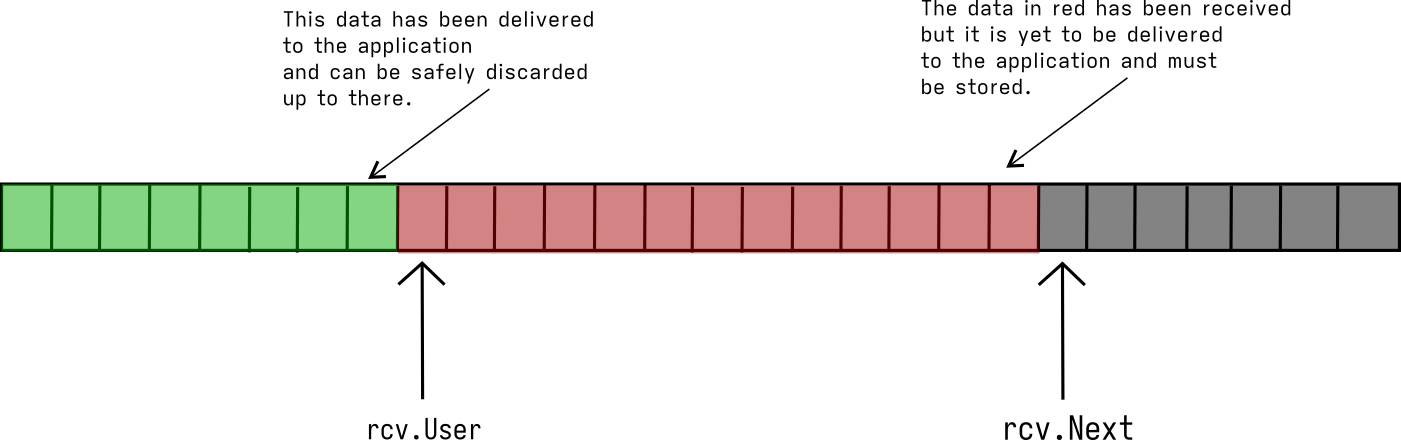
\includegraphics[ width=1.0\linewidth, height=\textheight, keepaspectratio]{./pics/tcp/RxBuffer.png}
	\caption{RX-buffer and its pointers.}
        \label{fig:RxBuffer}
\end{figure}



\section{Handling duplicates and loss}

IP is an unreliable protocol. This means that \emph{packets can be loss}.
Necessary mechanisms are

\begin{itemize}
	\item \textbf{retransmission};
	\item \textbf{acknowledgement}, which is a kind of \emph{notification
		of receipt}, in order to be sure that the receiver has received
		all the data we sent them.
\end{itemize}

Acknowledgements is a mechanism that assures receipt of a message by
notifications. Every header of a segment contains the sequence number of
\texttt{snd.Next}. Every segment also \emph{carries an information regarding
the bytes that are received}: the \textbf{acknowledgement number}, which tracks
the state of the RX-buffer by the pointer \texttt{rcv.Next}. This way, having
both sequence number and acknowledgement number, one can successfully track the
state of a TCP connection. When sending a TCP segment, both sequence number and
acknowledgement number are sent, so that the receiver can reconstruct the state
of the sender RX-buffer.

A fifth variable is needed: \texttt{snd.Ack}, which \emph{points to the byte in
TX-buffer that are both transmitted and acknowledged}. This variable is only
increased upon receiving data (for instance, upon receiving a sequence with a
greater ACK number from the sender). Data before \texttt{snd.Ack} pointer can
safely be discarded. Acknowledgements are crucial to a TCP connection, in order
to guarantee \textbf{reliability} of a connection (TCP is connection-oriented).
Therefore, transmission is always necessary even if TX-buffer is empty. That
case, no payload will be transmitted, only information in header is sent
(increasing acknowledgement number). 

Data bytes between pointers \texttt{snd.Ack} and \texttt{snd.Next} is said to
be \emph{in flight} data. These bytes have been transmitted but not yet
acknowledged.

\begin{figure}[b]
        \centering
        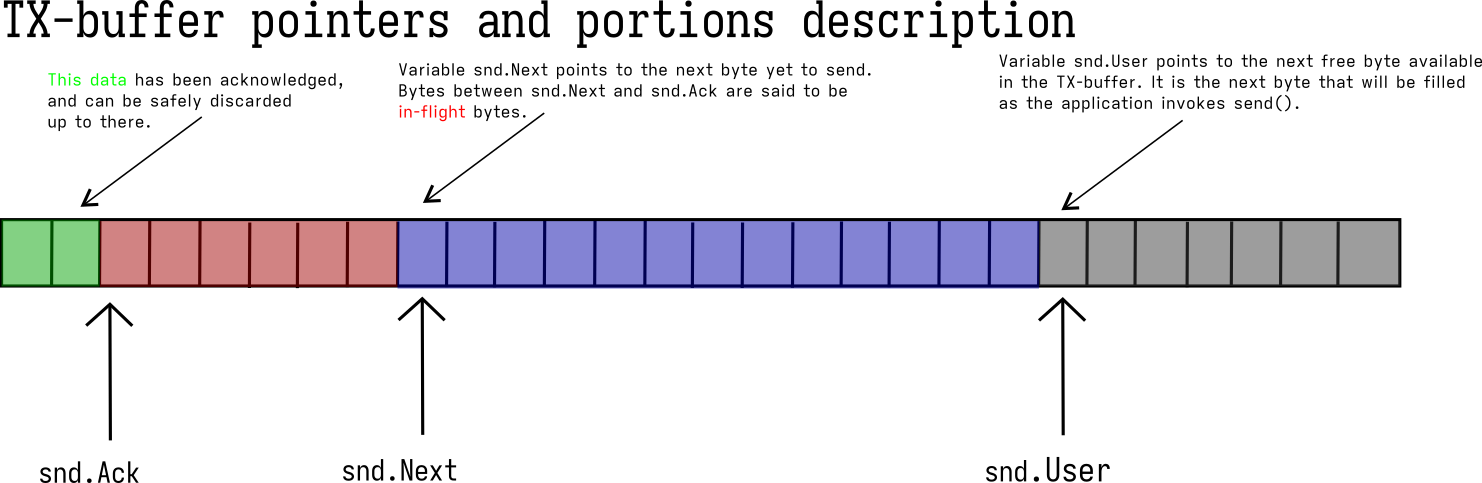
\includegraphics[ width=1.0\linewidth, height=\textheight, keepaspectratio]{./pics/tcp/TxBuffer.png}
	\caption{TX-Buffer and its flags \texttt{snd.Ack}, \texttt{snd.Next} and \texttt{snd.User}.}
        \label{fig:TxBuffer}
\end{figure}



\section{Delayed Acknowledgement}

\emph{Delayed Acknowledgement} is a famous TCP algorithm. It is pretty
straightforward:

\begin{quote}
Upon receiving a segment, if delayed-ack timer $T$ has previously been set,
transmit immediately. Else, set the delayed-ack timer $T$ to a value.
\end{quote}

Delayed-ack timer value depends on the operating system:

\begin{itemize}
	\item RFC suggests $T = 500ms$;
	\item Windows has $T = 200ms$;
	\item Linux in general has $T = 40ms$;
	\item RHEL sets $T = 4ms$.
\end{itemize}

If there is not much data to transmit, it will be likely that the timer $T$
will expire. If the other part is sending a lot of data, the contrary will be
more likely to occur, breaking the awaiting.

The core idea is to minimize the number of segments to be sent. In fact, a
delay time $T$ assured to save sending some segments, a feature that
historically was of a crucial importance.

\section{Retransmissions}

The connection state includes three more variables:

\begin{itemize}
	\item a \textbf{retransmission timer};
	\item a \emph{variable that describes the duration of retransmission
		timer}, the \textbf{RTO};
	\item a \textbf{retransmission counter}.
\end{itemize}

The algorithm is as follows:

\begin{quote}
Upon transmitting segment S, the counter is cleared and set to $0$, with the
timer set to the RTO value. Upon receiving an ACK, \texttt{snd.Ack} is set to
the maximum value between \texttt{snd.Ack} and \texttt{segment.Ack}. If
\texttt{snd.Ack == snd.Next} the timer is switched off.

When timer expires, the counter is incremented and if the counter has not yet
reached a \texttt{MAX\_COUNT} value, the segment is retransmitted. However, this
time the timer value is set to RTO but \texttt{RTO = 2 * RTO}. Only in-flight data
should be retransmitted (and all of it after timer expires). Basically, data
for which we are sure that it has been received, should not be retransmitted in
case the timer expires.

When counter reached \texttt{MAX\_COUNT} value, connection is closed.

A particular condition is when an ACK arrives for a portion of the data that
has been sent. In that case, the timer resets (the receiver has responded) and
the sender awaits ACK for missing segments.
\end{quote}

Windows closes connection after $5$ failed attempts, Linux after $15$.

It is simple to realise that there may be a lot of unnecessary retransmissions.
The timer can, for instance, run out too soon for the acknowledgement to reach
the sender. Unnecessary retransmissions are a waste of resources, a fundamental
problem. The reason could be one of those:

\begin{itemize}
	\item segments are lost;
	\item segments wich ACK are lost;
	\item RTO was set to a too small value.
\end{itemize}

Thus, RTO should be set to an appropriate value, since a too short value leads
to high overhead and possibly many unnecessary retransmissions, while a too
long value results in high latency and possibly a slow connection. RTO should
be set \textbf{dinamically}. The RTO should be slightly greater than the
\emph{RTT} (round-trip-time), and it is an idea from Jacobson algorithm. This
is of a crucial importance for TCP to work. Initial RTO value is heuristical,
and varies from one OS to another. Linux and Window start from same value,
macOS use a different value, and so on.

\section{Multiple default gateways}

More default gateways could be added to a single node. Reasons to add more than
one default gateway all boil up to failure avoidance. To know whether a gateway
has stopped working, a heuristic TCP algorithm tries gateway failure detection:

\begin{quote}
	if the number of retransmissions is greater than a \texttt{MAX\_COUNT}
	divided by 2 number, the \emph{connection} changes its default gateway.
	Moreover, if the number of connection that changed default gateway is
	greater than the number of open connections divided by 4, the \emph{IP
	layer} changes the default gateway. This last feature speeds up
	reconfiguration of early connections that still have to make some
	retransmission attemps.
\end{quote}

Basically, each connection can autonomously choose its own gateway, but the IP
layer can force any \--- new or already present \--- connection to use a
different default gateway.

\section{Gaps in RX-buffer}

Suppose that 4 segments are sent, but the second one has been lost. In this
case, the receiver has got all segments except the second one, however it has
no method to inform the sender to retransmit only the second segment. Sending
ACK for only the first segment would result in unnecessary retransmission of
segments 3 and 4. The receive buffer could end up having some \textbf{gaps},
missing bytes that are supposed to be received. The solutions are
\emph{Selective Acknowledgements} (SACK), a special kind of acknowledgements
that carry both \emph{left and right sequence number edges} of each
out-of-order \textbf{block} in RX-buffer, this way avoiding unnecessary
retransmissions. SACK protocol must be supported by both members of a
connection.

SACK is very convenient, since many segments can be lost when a sender tries to
deliver dozens of segments at once. This way, TCP can achieve \emph{efficient
handling} of the connection.

Of course, out-of-order segments could still lead to gaps in RX-buffer. In this
case, unnecessary retransmissions are unavoidable when an out-of-order segment
reaches the receiver too late (however, SACK reduces a lot the burden to the
sender since only missing segments should selectively be sent).

\section{Operating System TCP interrupts}

Upon packet arrival, a \emph{system interrupt} is sent. 

\chapter{Flow and Congestion Control}

Whenever TCP decides to transmit, there are three possible cases: 
\begin{itemize}
	\item an empty segment is sent when there is no payload;
	\item transmits a single segment if payload data is smaller than MSS;
	\item transmits multiple segments if paylod size exceeds MSS.
\end{itemize}

TCP initially starts slowly, then \emph{increases its transfer speed} according
to the rate in which acknowledgements are received. The overall interaction is
bidirectional and quite complicated, since TCP implementation at sender's side
tries to adapt to both connection properties and receiver's side properties.
As a general rule, the number of in-flight bytes is always lower than an upper
bound that is dynamically updated \--- this way, TCP can \emph{adapt} to the
peculiar characteristics of the connection and receiver's speed. Naturally
speaking, a sender should not send more segments than how many can be managed
by the receiver.

There are two different bounds and algorithms, the \textbf{flow control} and
\textbf{congestion control}. The first algorithm constructs a bound in such a
way that the capacity of the receiver is always respected. Let an extremely
fast computer send data faster than a receiving, slow, computer. Slower
computer has not enough speed to collect all data that has been sent \--- the
flow control algorithm lets the sender speed adapt to the receiver speed by
means of a \emph{send window}. The second algorithm, the congestion control,
constructs a state variable called \emph{congestion window} that . The number
of in-flight bytes \emph{must be slower than both send window and congestion
window multiplied by MSS}, so that $$\mbox{in-flight} \leq min(\mbox{sndWin},
\mbox{congWin} \cdot \mbox{MSS}).$$ Basically, if the transmission buffer is full of data,
a number of in-flight bytes equal to the minumum of both quantities should be
sent, otherwise just send \texttt{snd.User - snd.Ack} bytes (those still to
send).

\section{Managing memory buffers}

Buffers cannot increase indefinitely: boundaries must be set in order to assure
system stability. In Linux kernel, buffer size are set upon compilation.
Application should be suspended in case data cannot be pushed to TX-buffer (the
case when the buffer is full). When the RX-buffer is full, packets have to be
discarded since they cannot be collected. Flow control will act to prevent this
situation by letting the sender know how much free space is available to the
RX-buffer.

\section{Flow control}

Flow control is keeping a fast transmitter from overrunning a slower receiver.

Since application sends much data and faster than ACK arrive, the TX-buffer
could end up being filled up. At receiver's side, application invokes
\texttt{receive()} much slower than incoming packages speed. This way, the
RX-buffer could fill up as well. To solve this issues, application invokes
\texttt{send()} only when TX-buffer is full, hence it is put to sleep (blocked)
until TCP gets proper ACK and advances \texttt{snd.Ack} (when it has more free
space). TCP sender keeps track of free space in other end's RX-buffer by
looking at a variable in header that informs it of how much free space is
available, so that it can predict how much free space there is. When it guesses
that receiver's RX-buffer could be full and have no space available, it stops
transmission and suspends the application. If the maximum window corresponds to
the size of a single segment, the protocol is called \textbf{stop-and-wait}.
Larger windows enable pipelining of multiple segments in a row, enabling far
more efficient usage of the connection.

Flow control algorithm adopts the concept of \textbf{sliding window}. Each
segment header has a \texttt{WindowSize} field in the header that contains
\emph{how many free bytes are in the RX-buffer}. WindowSize field basically is
the amount of free space available in RX-buffer. At sending side,
\texttt{snd.winSize} contains the \emph{number of free bytes in RX-buffer of
the other side}. Initially it is set to the receiver's buffer size, and it is
updated dynamically upon sending a segment. If \texttt{S.Ack} is greater or
equal to \texttt{snd.Ack}, then the variable \texttt{snd.winSize} is set to
\texttt{S.windowSize}. Basically, the number of in-flight bytes must never
exceed the number of bytes in \texttt{snd.winSize} that are available in the
RX-buffer. The goal of TCP is to reach a number of in-flight bytes that is as
close as possible to the \texttt{snd.winSize} number of bytes, in order to
optimize the connection efficiently.

\subsection{Example: M * MSS window size and no transmission errors during flow}

\end{document}

